\documentclass[11pt,letterpaper]{article}

\usepackage{tabularx}
\usepackage{booktabs}
\usepackage{caption}
\usepackage[usenames, dvipsnames]{color}
\usepackage{subcaption}
\usepackage{setspace}
\usepackage{hyperref}
\usepackage{multirow}
\usepackage{minted}
\usepackage{mdframed}
\usepackage{lineno}
\usepackage{fullpage}
\linenumbers
\usepackage{pslatex}
% \usepackage{apacite}
\usepackage{graphicx}
\usepackage[margin=1.0in]{geometry}
\usepackage{pgfplots}
\usepackage{xcolor, colortbl}
\hypersetup{
    colorlinks,
    linkcolor={cyan!20!red},
    urlcolor={cyan!80!green},
    citecolor={cyan!80!blue}
}

\definecolor{light-gray}{HTML}{F0F0F0}

\usepackage{gb4e}  % linguistic examples
\noautomath

\usepackage{amsmath}

\newcommand{\pdone}{\tau_1^*}
\newcommand{\pdtwo}{\tau_2^*}
\newcommand{\pds}{(\pd1, \pd2)}
\newcommand{\fg}{f_{ground}}
\newcommand{\fe}{f_{excited}}

\doublespace

\title{Using a neural network to classify metaphorical/non-metaphorical violence on
cable news}

% \author{{\bf Matthew A.~Turner and Eshita Nandini}}

\begin{document}

\maketitle


\section{Introduction}\label{introduction}

Metaphor is often thought of as a decorative instrument of literature.
It is more scientifically productive to understand metaphor a basic
human cognitive capacity to represent relationships between concepts.
Mathematics, for example, may be understood as an elaborate metaphorical
scaffolding where ``embodied'' concepts are everywhere, such as the idea
that \(e^{i\theta}\) rotates a point in the complex plane by \(\theta\)
radians. Rotation is something we do every time we drive a car, so in
that way \(e^{i\theta}\) is physically intuitive because we have been
rotating different physical objects our entire lives \cite{Nunez1999, Núñez2000}. 
The
focus of this paper is not the metaphors of heavenly mathematics, but
messy metaphorical violence (MV) on cable news surrounding presidential
elections. Specifically, we present a neural network classifier for
determining whether or not a phrase is MV or not. This effort is an
important part of a larger effort to improve the throughput of an
existing metaphor annotation software application we are developing
called \emph{Metacorps} \cite{Turner2016}. Knowing what metaphors are said and
when in a society is important because metaphors are representations of
a society's conceptual relationships. Large-scale observations of
metaphor use are currently limited because it is a time-intensive task
for humans to do. We demonstrate that even with a modest gold-standard
dataset, a neural network system can distinguish, to around 85\%
accuracy, MV from non-MV. After introducing the motivation, we present
the data, our methods, and analyze the performance of some candidate
neural network classifiers. We close with a discussion of the promise
and challenges of integrating this system with teams of human
annotaters.

Evidence is growing that choice of metaphor, or whether or not to use
metaphor, has real consequences on cognition and behavior in general
\cite{Lakoff2014} and for politics \cite{Matlock2012}. 
A recent behavioral experiment showed more specifically that 
metaphorical violence 
Metaphor use is revealing:
spoken metaphors are either representative of the speaker's conceptual
system, or they are intended to cause the hearer to activate the metaphor's
conceptual links, or both.
So, if you want people to take climate change more seriously, you would
do better to frame it as a ``war'' instead of a ``race'' \cite{Flusberg2017}.

Results such as these are criticized for various reasons. 
One shortcoming is that in these studies are
cultural context is not part of the experiment. Linguists 
are increasingly looking to cultural context as
an important factor for explaining metaphor use \cite{Kovecses2010}. 
Another criticism
says we should not be asking ``if'' choice of metaphor influences
reasoning, but ``when'' does a particular metaphor have a causal effect
on reasoning \cite{Steen2014}? The contribution presented here helps solve
this contextual shortcoming, in that our data is timeseries data, so
current events such as the presidential debates are happening in the
cultural background. Further context is ideological context, with cable
news channel as proxy for ideology \cite{Mitchell2014, King2017}. Taken more
generally, the context is English-speaking American cable television news.
Our analysis enables us to observe how metaphorical violence varies between 
cable news networks.

An example metaphorical phrase might be the headline ``Bernie attacks
Clinton Foundation in first debate.'' On the contrary, ``Terrorist attack kills
US Ambassador to Libya'' is clearly not a metaphor. Metaphor serves a pragmatic
purpose: it is a much shorter, if incomplete, version of what might be
the non-metaphorical way to explain that actually ``Bernie claimed that
the Clinton Foundation had wrongly accepted funds.'' In a concurrent
project, we have developed and fit a simple dynamical model to the
frequency of metaphorical violence (MV) use, and found that MV usage
increases in frequency for all networks, but with different timing in
2012 and 2016.

While we are able to get novel and interesting results with
human-generated annotations, machine learning could help us increase our
signal power. For the study just mentioned, in 2012 and 2016 we had to
limit our corpus to include only the top two most-watched shows on each
of the three networks. As mentioned, we limited ourselves there to three
violent words. This is because manual annotation is a time-consuming
process. Often, relevant parts of the episode must be watched to finish
an annotation, which currently requires navigation of the TVNA website.
The first use of Metacorps was to increase the efficacy of human coders
by streamlining the annotation process. But by building our own
annotation web application and data model, we can incorporate a new
service whose prototype is introduced in this report: a neural network
that classifies potential metaphorical violence as metaphor or not. The
next section details the machine learning task, describes the gold
standard dataset and the training/validation/test datasets.

\section{Data}\label{data}

Metacorps provides a data model and web interface for annotating
metaphor in a corpus. In its present state, all corpora are
pre-processed subcorpora of the closed captions hosted and curated by
the TV News Archive. The TV News archive
\url{http://archive.org/tv/details} provides video, audio, closed
captioning, and rich metadata for millions of hours of television news
from cable news channels, studied here, and local news. They provide an
HTTP API that provides JSON search results and episode metadata. To be
specific, \emph{episode} refers to a single showing of a particular
show, like \emph{The O'Reilly Factor}. Reruns are independent episodes
and must be excluded. A show's metadata includes links to its data,
which may be in the form of video, audio, or closed captions. This study
uses the closed captions. To programatically acquire data and build
transcripts from closed captionings we used Python software
\texttt{iatv} available on GitHub \cite{Turner2016}.

Gold standard annotations were created using the Metacorps Python
software package and web application \cite{Turner2017}. Trained annotators
use the web application to indicate which phrases of potential metaphor
actually are metaphor, then fill in more information, such as who the
subject and object are of the metaphorical violence. Potential instances
of metaphorical violence are found by searching for key violent words;
in this study those words are \emph{hit}, \emph{beat}, and
\emph{attack}. The corpus we searched was of transcripts from the top
two shows on each of the three cable networks MSNBC, CNN, and Fox News from
the months September to November, 2012. 

To build the corpus, we used \textit{iatv} to download the transcripts from
the desired shows in the desired timeframe. \textit{Metacorps} provides 
a data model built on MongoDB and its object-document mapper mongoengine for
Python. Transcripts and other metadata are persisted. Other elements in the
data model provide fields to annotate these base transcripts, which are
linked. Human annotaters have suggested and agreed upon whether or not a
phrase is metaphorical violence. See Figure \ref{fig:metacorps} for a
sketch of the Metacorps data flow and where our new classifier fits in.
Metacorps also provides a data exporter that
created the gold standard dataset 
\href{http://metacorps.io/static/data/viomet-2012.csv}{viomet-2012.csv} used
to train, validate, and test our model.

\begin{figure}
  \centering
  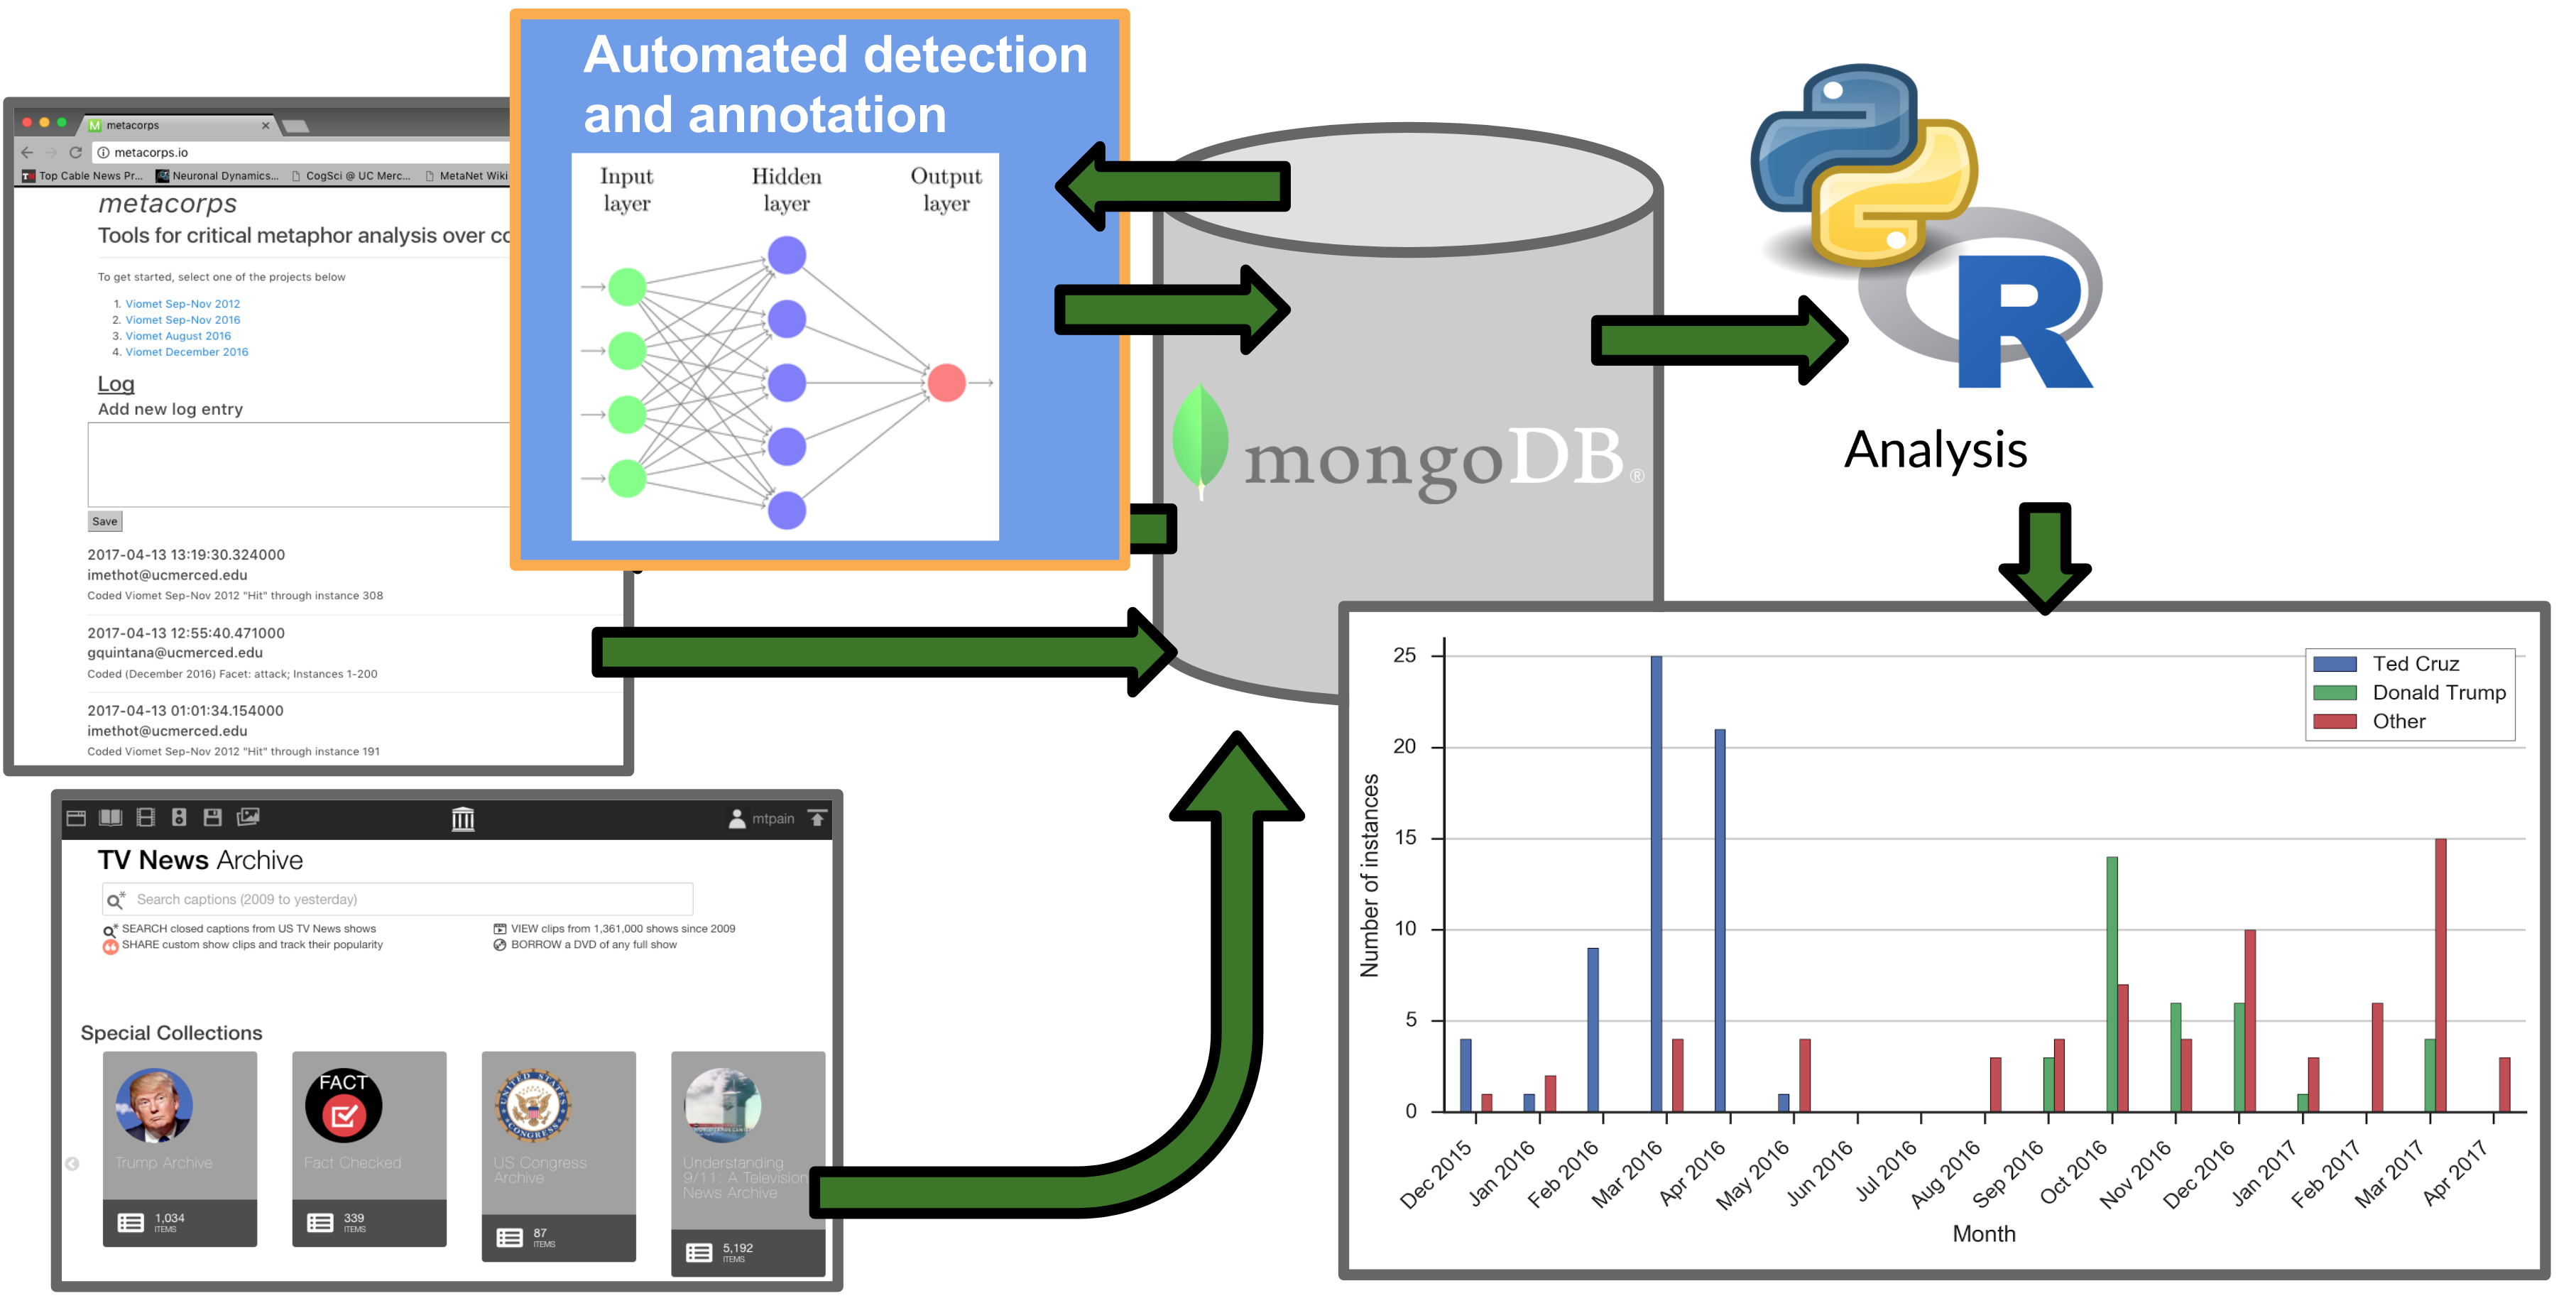
\includegraphics[width=.9\textwidth]{Figures/metacorps-schematic}
\caption{Schematic of Metacorps: the annotation toolset that connects 
  cable news transcripts to annotators, annotations to meaningful data tables, 
  and soon annotations and analyses to our neural network classifier.}
\label{fig:metacorps}
\end{figure}


\section{Methods}\label{methods}

To accomplish this MV classification task, we experimented with deep
feedforward neural networks, encouraged by success on a similar task reported in
\cite{DoDinh2016}. Each hidden layer had 500 nodes, and we
tested 1-, 2-, 4-, and 6-hidden-layer models. To regularize we use
dropout and early stopping. Stochastic gradient descent with momentum
minimized the cross entropy loss. The inputs were vectors with 3300
elements: eleven words represented by their word2vec embeddings, which
come from the GoogleNews pre-trained word2vec (download here:
\url{https://github.com/mmihaltz/word2vec\-GoogleNews\-vectors/raw/master/GoogleNews\-vectors\-negative300.bin.gz})
Each word embedding vector is concatenated with the next to create the
network input vector. We used the free and open source Python package 
\texttt{gensim} for loading the binary-formatted word embeddings \cite{Rehurek2010}.
Neural network construction, training, and testing was done primarily in
\href{https://www.tensorflow.org/}{TensorFlow} \cite{}. Performance 
analysis was done using Scikit-Learn, and table reading, writing, and 
subsetting was done with Pandas. More details can be found by examining the
README and code for 
\href{https://github.com/mtpain/math292-fall17-project}{this project on GitHub}.

To investigate the performance of the different hyperparameterizations over
the number of layers and the learning rate, we executed twenty trials for
every combination of the number of layers (1, 2, 4, or 6) and learning rate
(0.01, 0.1, or 0.5). To do this we utilized the MERCED computing cluster hosted
at UC Merced. We then calculated the average precision, sensitivity, specificity,
and AUC for each of these; the results are presented in Table~\ref{tab:main}.

\section{Results}\label{results}

Results go here!
% \input{Table.tex}

\section{Discussion}\label{discussion}

\begin{itemize}
  \item Different word vectors. For example, choice of embeddings has been
    shown to influence another metaphor identification task \cite{Rei2017}.
    What if we built word embeddings from the corpora itself?
  \item More hyperparameters: window size, number of nodes per layer, learning
    rate.
  \item Other architectures: convolutional neural net since the word window
    is really 2-dimensional. LSTM? "Supervised similarity network" was 
    proposed and tested in \cite{Rei2017}, but this operated on word pairs,
    which for us often would not be enough: ``attacked her'', ``to hit'', and
    so on would be very frequent and low on information.
  \item Other representations of words and sentences.
  \item Lessons or opportunities for cognitive science? Model of the neural
    theory of metaphor?
  \item Select the best-performing trained model of the best hyperparameters and
inspect it in more detail. Specifically, we investigate performance for 
subsets of the test set based on which violent word was used. 
\end{itemize}

\bibliographystyle{unsrt}
\bibliography{/Users/mt/workspace/papers/library.bib}

\end{document}
